\documentclass{article}

% content/resources/templates/preamble.tex
\usepackage[margin=0.6in]{geometry}
\author{Milav Dabgar}
\usepackage{amsmath,amssymb,amsthm}
\usepackage{booktabs}
\usepackage{multirow}
\usepackage{xcolor}
\usepackage{tcolorbox}
\tcbuselibrary{breakable,skins}
\usepackage[colorlinks=true,linkcolor=blue]{hyperref}
\usepackage{titlesec}
\usepackage{enumitem}
\usepackage{tikz}
\usepackage{pgfplots}
\usepackage{circuitikz}
\usepackage[version=4]{mhchem}
\usepackage{longtable}
\usepackage{array}
\usepackage{float}
\usepackage{caption}
\usepackage{listings}

\lstset{
  basicstyle=\small\ttfamily,
  breaklines=true,
  breakatwhitespace=false,
  postbreak=\mbox{\textcolor{red}{$\hookrightarrow$}\space},
  float=false,
  numbers=left,
  numberstyle=\tiny\color{gray},
  numbersep=10pt,
  xleftmargin=2em,
  keywordstyle=\color{blue},
  commentstyle=\color{green!60!black},
  stringstyle=\color{purple},
  backgroundcolor=\color{gray!5},
  showstringspaces=false,
  tabsize=2,
  captionpos=b,
  keepspaces=true,
  columns=flexible
}

\pgfplotsset{compat=1.18}
\usetikzlibrary{shapes,arrows,positioning,calc,patterns,decorations.pathmorphing,decorations.markings,arrows.meta}

% Color scheme
\definecolor{headcolor}{RGB}{0,102,204}
\definecolor{keycolor}{RGB}{220,20,60}
\definecolor{solutioncolor}{RGB}{34,139,34}
\definecolor{mnemoniccolor}{RGB}{148,0,211}
\definecolor{codecolor}{RGB}{0,0,100}

% Spacing
\setlength{\parskip}{3pt}
\setlist[itemize]{nosep}
\setlist[enumerate]{nosep}

% Title formatting
\titleformat{\section}{\Large\bfseries\color{headcolor}}{\thesection}{1em}{}
\titleformat{\subsection}{\large\bfseries\color{headcolor}}{\thesubsection}{1em}{}

% Pandoc tightlist compatibility
\providecommand{\tightlist}{%
  \setlength{\itemsep}{0pt}\setlength{\parskip}{0pt}}

% Pandoc longtable compatibility
\newcounter{none}
\def\thenone{}


% content/resources/templates/english-boxes.tex

% Custom environments
\newtcolorbox{solutionbox}{
 breakable,
 enhanced,
 colback=solutioncolor!5!white,
 colframe=solutioncolor!75!black,
 fonttitle=\bfseries,
 title=Solution
}

\newtcolorbox{solutionboxnobreak}{
 colback=solutioncolor!5!white,
 colframe=solutioncolor!75!black,
 fonttitle=\bfseries,
 title=Solution
}

\newtcolorbox{keyformula}{
 breakable,
 enhanced,
 colback=keycolor!5!white,
 colframe=keycolor!75!black,
 fonttitle=\bfseries,
 title=Key Formula
}

\newtcolorbox{mnemonicboxenv}{
 breakable,
 enhanced,
 colback=mnemoniccolor!5!white,
 colframe=mnemoniccolor!75!black,
 fonttitle=\bfseries,
 title=Mnemonic
}

\newcommand{\mnemonicbox}[1]{%
  \begin{mnemonicboxenv}
    #1
  \end{mnemonicboxenv}
}


% Custom commands for GTU solutions
% This file defines semantic commands for consistent formatting

% Question command with automatic formatting
\newcommand{\question}[2]{%
  \section*{Question #1}%
  \textbf{#2}%
}

% OR question variant
\newcommand{\questionor}[2]{%
  \section*{Question #1 OR}%
  \textbf{#2}%
}

% Proper table environment with caption
\newenvironment{answertable}[1]{%
  \begin{table}[htbp]
  \centering
  \caption{#1}
}{%
  \end{table}
}

% Proper figure environment for diagrams
\newenvironment{answerdiagram}[1]{%
  \begin{figure}[htbp]
  \centering
  \caption{#1}
}{%
  \end{figure}
}

% Semantic markup for key terms
\newcommand{\keyword}[1]{\textbf{#1}}
\newcommand{\code}[1]{\texttt{#1}}
\newcommand{\classname}[1]{\texttt{#1}}
\newcommand{\methodname}[1]{\texttt{#1}}

% Proper quotation marks
\newcommand{\mnemonic}[1]{``#1''}


\title{Foundation of AI and ML (4351601) - Winter 2023 Solution}
\author{Milav Dabgar}
\date{December 04, 2023}

\begin{document}
\maketitle

\questionmarks{1}{a}{3}
\textbf{Define the following terms: (1) Artificial Intelligence (2) Expert System.}

\begin{solutionbox}
    \begin{tabulary}{\linewidth}{L L}
        \hline
        \textbf{Term} & \textbf{Definition} \\
        \hline
        \textbf{Artificial Intelligence} & AI is a branch of computer science that creates machines capable of performing tasks that typically require human intelligence, such as learning, reasoning, and problem-solving. \\
        \textbf{Expert System} & An expert system is a computer program that uses knowledge and inference rules to solve problems that normally require human expertise in a specific domain. \\
        \hline
    \end{tabulary}

    \begin{itemize}
        \item \textbf{AI characteristics}: Learning, reasoning, perception
        \item \textbf{Expert system components}: Knowledge base, inference engine
    \end{itemize}

    \begin{mnemonicbox}
    "AI Learns, Expert Advises"
\end{mnemonicbox}
\end{solutionbox}

\questionmarks{1}{b}{4}
\textbf{Compare Biological Neural Network and Artificial Neural Network.}

\begin{solutionbox}
    \begin{tabulary}{\linewidth}{L L L}
        \hline
        \textbf{Aspect} & \textbf{Biological Neural Network} & \textbf{Artificial Neural Network} \\
        \hline
        \textbf{Processing} & Parallel processing & Sequential/parallel processing \\
        \textbf{Speed} & Slow (milliseconds) & Fast (nanoseconds) \\
        \textbf{Learning} & Continuous learning & Batch/online learning \\
        \textbf{Storage} & Distributed storage & Centralized storage \\
        \hline
    \end{tabulary}

    \begin{itemize}
        \item \textbf{Biological}: Complex, fault-tolerant, self-repairing
        \item \textbf{Artificial}: Simple, precise, programmable
    \end{itemize}

    \begin{mnemonicbox}
    "Bio is Complex, AI is Simple"
\end{mnemonicbox}
\end{solutionbox}

\questionmarks{1}{c}{7}
\textbf{Explain types of AI with its applications.}

\begin{solutionbox}
    \begin{tabulary}{\linewidth}{L L L}
        \hline
        \textbf{Type of AI} & \textbf{Description} & \textbf{Applications} \\
        \hline
        \textbf{Narrow AI} & AI designed for specific tasks & Voice assistants, recommendation systems \\
        \textbf{General AI} & AI with human-level intelligence & Not yet achieved \\
        \textbf{Super AI} & AI exceeding human intelligence & Theoretical concept \\
        \hline
    \end{tabulary}

    \begin{figure}[H]
        \centering
        \begin{tikzpicture}[node distance=2cm, auto]
            \node [gtu block] (types) {Types of AI};
            \node [gtu block, below left=of types] (narrow) {Narrow AI};
            \node [gtu block, below=of types] (general) {General AI};
            \node [gtu block, below right=of types] (super) {Super AI};
            
            \node [gtu state, below=0.5cm of narrow] (narrow_app) {Siri, Alexa};
            \node [gtu state, below=0.5cm of general] (general_app) {Human-level};
            \node [gtu state, below=0.5cm of super] (super_app) {Beyond Human};

            \path [gtu arrow] (types) -- (narrow);
            \path [gtu arrow] (types) -- (general);
            \path [gtu arrow] (types) -- (super);
            \path [gtu arrow] (narrow) -- (narrow_app);
            \path [gtu arrow] (general) -- (general_app);
            \path [gtu arrow] (super) -- (super_app);
        \end{tikzpicture}
        \caption{Types of Artificial Intelligence}
    \end{figure}

    \begin{itemize}
        \item \textbf{Current focus}: Narrow AI dominates today's applications
        \item \textbf{Future goal}: Achieving General AI safely
    \end{itemize}

    \begin{mnemonicbox}
    "Narrow Now, General Goal, Super Scary"
\end{mnemonicbox}
\end{solutionbox}

\questionmarks{1}{c}{7}
\textbf{Explain AI ethics and limitations.}

\begin{solutionbox}
    \begin{tabulary}{\linewidth}{L L}
        \hline
        \textbf{Ethics Aspect} & \textbf{Description} \\
        \hline
        \textbf{Privacy} & Protecting personal data and user information \\
        \textbf{Bias} & Ensuring fairness across different groups \\
        \textbf{Transparency} & Making AI decisions explainable \\
        \textbf{Accountability} & Determining responsibility for AI actions \\
        \hline
    \end{tabulary}

    \textbf{Limitations:}
    \begin{itemize}
        \item \textbf{Data dependency}: Requires large, quality datasets
        \item \textbf{Computational power}: Needs significant processing resources
        \item \textbf{Lack of creativity}: Cannot truly create original concepts
    \end{itemize}

    \begin{mnemonicbox}
    "Privacy, Bias, Transparency, Accountability"
\end{mnemonicbox}
\end{solutionbox}

\questionmarks{2}{a}{3}
\textbf{Define the following terms: (1) Well posed Learning Problem (2) Machine Learning.}

\begin{solutionbox}
    \begin{tabulary}{\linewidth}{L L}
        \hline
        \textbf{Term} & \textbf{Definition} \\
        \hline
        \textbf{Well posed Learning Problem} & A learning problem with clearly defined task (T), performance measure (P), and experience (E) where performance improves with experience. \\
        \textbf{Machine Learning} & A subset of AI that enables computers to learn and improve automatically from experience without being explicitly programmed. \\
        \hline
    \end{tabulary}

    \begin{itemize}
        \item \textbf{Well posed formula}: T + P + E = Learning
        \item \textbf{ML advantage}: Automatic improvement from data
    \end{itemize}

    \begin{mnemonicbox}
    "Task, Performance, Experience"
\end{mnemonicbox}
\end{solutionbox}

\questionmarks{2}{b}{4}
\textbf{Explain Reinforcement Learning along with terms used in it.}

\begin{solutionbox}
    \begin{tabulary}{\linewidth}{L L}
        \hline
        \textbf{Term} & \textbf{Description} \\
        \hline
        \textbf{Agent} & The learner or decision maker \\
        \textbf{Environment} & The world in which agent operates \\
        \textbf{Action} & What agent can do in each state \\
        \textbf{State} & Current situation of the agent \\
        \textbf{Reward} & Feedback from environment \\
        \hline
    \end{tabulary}

    \begin{figure}[H]
        \centering
        \begin{tikzpicture}[node distance=2.5cm, auto]
            \node [gtu block] (agent) {Agent};
            \node [gtu block, right=4cm of agent] (env) {Environment};

            \path [gtu arrow, bend left] (agent) edge node {Action} (env);
            \path [gtu arrow, bend left] (env) edge node {State, Reward} (agent);
        \end{tikzpicture}
        \caption{Reinforcement Learning Cycle}
    \end{figure}

    \begin{itemize}
        \item \textbf{Learning process}: Trial and error approach
        \item \textbf{Goal}: Maximize cumulative reward
    \end{itemize}

    \begin{mnemonicbox}
    "Agent Acts, Environment States and Rewards"
\end{mnemonicbox}
\end{solutionbox}

\questionmarks{2}{c}{7}
\textbf{Compare Supervised, Unsupervised and Reinforcement Learning.}

\begin{solutionbox}
    \begin{tabulary}{\linewidth}{L L L L}
        \hline
        \textbf{Aspect} & \textbf{Supervised} & \textbf{Unsupervised} & \textbf{Reinforcement} \\
        \hline
        \textbf{Data} & Labeled data & Unlabeled data & Interactive data \\
        \textbf{Goal} & Predict output & Find patterns & Maximize reward \\
        \textbf{Feedback} & Immediate & None & Delayed \\
        \textbf{Examples} & Classification & Clustering & Game playing \\
        \hline
    \end{tabulary}

    \begin{itemize}
        \item \textbf{Supervised}: Teacher-guided learning
        \item \textbf{Unsupervised}: Self-discovery learning
        \item \textbf{Reinforcement}: Trial-and-error learning
    \end{itemize}

    \begin{mnemonicbox}
    "Supervised has Teacher, Unsupervised Discovers, Reinforcement Tries"
\end{mnemonicbox}
\end{solutionbox}

\questionmarks{2}{a}{3}
\textbf{Write Key features of Reinforcement Learning.}

\begin{solutionbox}
    \begin{tabulary}{\linewidth}{L L}
        \hline
        \textbf{Feature} & \textbf{Description} \\
        \hline
        \textbf{Trial and Error} & Learning through experimentation \\
        \textbf{Delayed Reward} & Feedback comes after actions \\
        \textbf{Sequential Decision} & Actions affect future states \\
        \hline
    \end{tabulary}

    \begin{itemize}
        \item \textbf{No supervisor}: Agent learns independently
        \item \textbf{Exploration vs Exploitation}: Balance between trying new actions and using known good actions
    \end{itemize}

    \begin{mnemonicbox}
    "Try, Delay, Sequence"
\end{mnemonicbox}
\end{solutionbox}

\questionmarks{2}{b}{4}
\textbf{Explain Types of Reinforcement learning.}

\begin{solutionbox}
    \begin{tabulary}{\linewidth}{L L}
        \hline
        \textbf{Type} & \textbf{Description} \\
        \hline
        \textbf{Positive RL} & Adding positive stimulus to increase behavior \\
        \textbf{Negative RL} & Removing negative stimulus to increase behavior \\
        \hline
    \end{tabulary}

    \textbf{Based on Learning:}
    \begin{itemize}
        \item \textbf{Model-based}: Agent learns environment model
        \item \textbf{Model-free}: Agent learns directly from experience
    \end{itemize}

    \begin{mnemonicbox}
    "Positive Adds, Negative Removes"
\end{mnemonicbox}
\end{solutionbox}

\questionmarks{2}{c}{7}
\textbf{Explain approaches to implement Reinforcement Learning.}

\begin{solutionbox}
    \begin{tabulary}{\linewidth}{L L L}
        \hline
        \textbf{Approach} & \textbf{Description} & \textbf{Example} \\
        \hline
        \textbf{Value-based} & Learn value of states/actions & Q-Learning \\
        \textbf{Policy-based} & Learn policy directly & Policy Gradient \\
        \textbf{Model-based} & Learn environment model & Dynamic Programming \\
        \hline
    \end{tabulary}

    \begin{figure}[H]
        \centering
        \begin{tikzpicture}[node distance=1.5cm, auto]
            \node [gtu block] (rl) {RL Approaches};
            \node [gtu block, below left=of rl] (value) {Value-based};
            \node [gtu block, below=of rl] (policy) {Policy-based};
            \node [gtu block, below right=of rl] (model) {Model-based};
            
            \node [gtu state, below=0.5cm of value] (qlearn) {Q-Learning};
            \node [gtu state, below=0.5cm of policy] (pgrad) {Policy Gradient};
            \node [gtu state, below=0.5cm of model] (dp) {Dynamic Prog.};

            \path [gtu arrow] (rl) -- (value);
            \path [gtu arrow] (rl) -- (policy);
            \path [gtu arrow] (rl) -- (model);
            \path [gtu arrow] (value) -- (qlearn);
            \path [gtu arrow] (policy) -- (pgrad);
            \path [gtu arrow] (model) -- (dp);
        \end{tikzpicture}
        \caption{Reinforcement Learning Approaches}
    \end{figure}

    \begin{itemize}
        \item \textbf{Value-based}: Estimates value functions
        \item \textbf{Policy-based}: Optimizes policy parameters
        \item \textbf{Model-based}: Uses environment model
    \end{itemize}

    \begin{mnemonicbox}
    "Value, Policy, Model"
\end{mnemonicbox}
\end{solutionbox}

\questionmarks{3}{a}{3}
\textbf{Describe the activation functions ReLU and sigmoid.}

\begin{solutionbox}
    \begin{tabulary}{\linewidth}{L L L}
        \hline
        \textbf{Function} & \textbf{Formula} & \textbf{Range} \\
        \hline
        \textbf{ReLU} & f(x) = max(0, x) & [0, $\infty$) \\
        \textbf{Sigmoid} & f(x) = 1/(1 + $e^{-x}$) & (0, 1) \\
        \hline
    \end{tabulary}

    \begin{itemize}
        \item \textbf{ReLU advantage}: No vanishing gradient problem
        \item \textbf{Sigmoid advantage}: Smooth gradient, probabilistic output
    \end{itemize}

    \begin{mnemonicbox}
    "ReLU Rectifies, Sigmoid Squashes"
\end{mnemonicbox}
\end{solutionbox}


\questionmarks{3}{b}{4}
\textbf{Explain Multi-layer feed forward ANN.}

\begin{solutionbox}
    \begin{tabulary}{\linewidth}{L L}
        \hline
        \textbf{Component} & \textbf{Description} \\
        \hline
        \textbf{Input Layer} & Receives input data \\
        \textbf{Hidden Layers} & Process information (multiple layers) \\
        \textbf{Output Layer} & Produces final result \\
        \textbf{Connections} & Forward direction only \\
        \hline
    \end{tabulary}

    \begin{itemize}
        \item \textbf{Information flow}: Unidirectional from input to output
        \item \textbf{No cycles}: No feedback connections
    \end{itemize}

    \begin{mnemonicbox}
    "Input \textrightarrow Hidden \textrightarrow Output (Forward Only)"
\end{mnemonicbox}
\end{solutionbox}

\questionmarks{3}{c}{7}
\textbf{Draw the structure of ANN and explain functionality of each of its components.}

\begin{solutionbox}
    \begin{figure}[H]
        \centering
        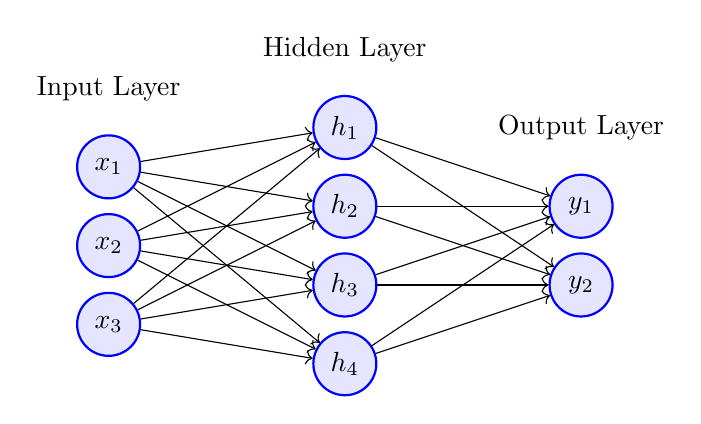
\begin{tikzpicture}[
            neuron/.style={circle, fill=blue!10, draw=blue, thick, minimum size=0.8cm}
        ]
            % Input Layer
            \node[neuron] (x1) at (0,2) {$x_1$};
            \node[neuron] (x2) at (0,1) {$x_2$};
            \node[neuron] (x3) at (0,0) {$x_3$};
            
            % Hidden Layer
            \node[neuron] (h1) at (3,2.5) {$h_1$};
            \node[neuron] (h2) at (3,1.5) {$h_2$};
            \node[neuron] (h3) at (3,0.5) {$h_3$};
            \node[neuron] (h4) at (3,-0.5) {$h_4$};
            
            % Output Layer
            \node[neuron] (y1) at (6,1.5) {$y_1$};
            \node[neuron] (y2) at (6,0.5) {$y_2$};
            
            % Connections from input to hidden
            \foreach \i in {1,2,3}
                \foreach \j in {1,2,3,4}
                    \draw[->] (x\i) -- (h\j);
            
            % Connections from hidden to output
            \foreach \i in {1,2,3,4}
                \foreach \j in {1,2}
                    \draw[->] (h\i) -- (y\j);
            
            % Labels
            \node[above=0.3cm of x1] {Input Layer};
            \node[above=0.3cm of h1] {Hidden Layer};
            \node[above=0.3cm of y1] {Output Layer};
        \end{tikzpicture}
        \caption{Artificial Neural Network Structure}
    \end{figure}

    \begin{tabulary}{\linewidth}{L L}
        \hline
        \textbf{Component} & \textbf{Functionality} \\
        \hline
        \textbf{Neurons} & Processing units that receive inputs and produce outputs \\
        \textbf{Weights} & Connection strengths between neurons \\
        \textbf{Bias} & Additional parameter to shift activation function \\
        \textbf{Activation Function} & Introduces non-linearity to the network \\
        \hline
    \end{tabulary}

    \begin{itemize}
        \item \textbf{Input layer}: Receives and distributes input data
        \item \textbf{Hidden layers}: Extract features and patterns
        \item \textbf{Output layer}: Produces final classification or prediction
        \item \textbf{Connections}: Weighted links between neurons
    \end{itemize}

    \begin{mnemonicbox}
    "Neurons with Weights, Bias, and Activation"
\end{mnemonicbox}
\end{solutionbox}

\questionmarks{3}{a}{3}
\textbf{Write a short note on Backpropagation.}

\begin{solutionbox}
    \begin{tabulary}{\linewidth}{L L}
        \hline
        \textbf{Aspect} & \textbf{Description} \\
        \hline
        \textbf{Purpose} & Training algorithm for neural networks \\
        \textbf{Method} & Gradient descent with chain rule \\
        \textbf{Direction} & Backward error propagation \\
        \hline
    \end{tabulary}

    \begin{itemize}
        \item \textbf{Process}: Calculate error gradients backwards through network
        \item \textbf{Update}: Adjust weights to minimize error
    \end{itemize}

    \begin{mnemonicbox}
    "Back-ward Error Propagation"
\end{mnemonicbox}
\end{solutionbox}

\questionmarks{3}{b}{4}
\textbf{Explain Single-layer feed forward network.}

\begin{solutionbox}
    \begin{tabulary}{\linewidth}{L L}
        \hline
        \textbf{Feature} & \textbf{Description} \\
        \hline
        \textbf{Structure} & Input layer directly connected to output layer \\
        \textbf{Layers} & Only input and output layers \\
        \textbf{Limitations} & Can only solve linearly separable problems \\
        \textbf{Example} & Perceptron \\
        \hline
    \end{tabulary}

    \begin{itemize}
        \item \textbf{Capability}: Limited to linear decision boundaries
        \item \textbf{Applications}: Simple classification tasks
    \end{itemize}

    \begin{mnemonicbox}
    "Single Layer, Linear Limits"
\end{mnemonicbox}
\end{solutionbox}

\questionmarks{3}{c}{7}
\textbf{Draw and explain the architecture of Recurrent neural network.}

\begin{solutionbox}
    \begin{figure}[H]
        \centering
        \begin{tikzpicture}[node distance=2cm, auto]
            \node [gtu block] (input) {Input};
            \node [gtu block, right=of input] (hidden) {Hidden State};
            \node [gtu block, right=of hidden] (output) {Output};
            
            % Feedback loop
            \path [gtu arrow] (input) -- (hidden);
            \path [gtu arrow] (hidden) -- (output);
            
            \draw [gtu arrow] (hidden.south) to [out=270,in=270,looseness=4] node[below]{Recurrent Connection} (hidden.south);

        \end{tikzpicture}
        \caption{Recurrent Neural Network Architecture}
    \end{figure}

    \begin{tabulary}{\linewidth}{L L}
        \hline
        \textbf{Component} & \textbf{Function} \\
        \hline
        \textbf{Hidden State} & Maintains memory of previous inputs \\
        \textbf{Recurrent Connection} & Feedback from hidden state to itself \\
        \textbf{Sequence Processing} & Handles sequential data \\
        \hline
    \end{tabulary}

    \begin{itemize}
        \item \textbf{Memory}: Retains information from previous time steps
        \item \textbf{Applications}: Language modeling, speech recognition
        \item \textbf{Advantage}: Can process variable-length sequences
    \end{itemize}

    \begin{mnemonicbox}
    "Recurrent Remembers, Loops Back"
\end{mnemonicbox}
\end{solutionbox}

\questionmarks{4}{a}{3}
\textbf{Define NLP and write down advantages of it.}

\begin{solutionbox}
    \begin{tabulary}{\linewidth}{L L}
        \hline
        \textbf{Term} & \textbf{Definition} \\
        \hline
        \textbf{NLP} & Natural Language Processing - enables computers to understand, interpret, and generate human language \\
        \hline
    \end{tabulary}

    \textbf{Advantages:}
    \begin{itemize}
        \item \textbf{Human-computer interaction}: Natural communication
        \item \textbf{Automation}: Automated text processing and analysis
        \item \textbf{Accessibility}: Voice interfaces for disabled users
    \end{itemize}

    \begin{mnemonicbox}
    "Natural Language, Natural Interaction"
\end{mnemonicbox}
\end{solutionbox}

\questionmarks{4}{b}{4}
\textbf{Compare NLU and NLG.}

\begin{solutionbox}
    \begin{tabulary}{\linewidth}{L L L}
        \hline
        \textbf{Aspect} & \textbf{NLU (Understanding)} & \textbf{NLG (Generation)} \\
        \hline
        \textbf{Purpose} & Interpret human language & Generate human language \\
        \textbf{Input} & Text/Speech & Structured data \\
        \textbf{Output} & Structured data & Text/Speech \\
        \textbf{Examples} & Sentiment analysis & Text summarization \\
        \hline
    \end{tabulary}

    \begin{itemize}
        \item \textbf{NLU}: Converts unstructured text to structured data
        \item \textbf{NLG}: Converts structured data to natural text
    \end{itemize}

    \begin{mnemonicbox}
    "NLU Understands, NLG Generates"
\end{mnemonicbox}
\end{solutionbox}

\questionmarks{4}{c}{7}
\textbf{Explain word tokenization and frequency distribution of words with suitable example.}

\begin{solutionbox}
    \begin{tabulary}{\linewidth}{L L L}
        \hline
        \textbf{Process} & \textbf{Description} & \textbf{Example} \\
        \hline
        \textbf{Tokenization} & Breaking text into individual words/tokens & "Hello world" \textrightarrow ["Hello", "world"] \\
        \textbf{Frequency Distribution} & Counting occurrence of each token & \{"Hello": 1, "world": 1\} \\
        \hline
    \end{tabulary}

    \textbf{Example:}
    \begin{lstlisting}
Text: "The cat sat on the mat"
Tokens: ["The", "cat", "sat", "on", "the", "mat"]
Frequency: {"The": 1, "cat": 1, "sat": 1, "on": 1, "the": 1, "mat": 1}
    \end{lstlisting}

    \begin{itemize}
        \item \textbf{Case sensitivity}: "The" and "the" counted separately
        \item \textbf{Applications}: Text analysis, search engines
        \item \textbf{Preprocessing}: Essential step for NLP tasks
    \end{itemize}

    \begin{mnemonicbox}
    "Tokenize then Count"
\end{mnemonicbox}
\end{solutionbox}

\questionmarks{4}{a}{3}
\textbf{List disadvantages of NLP.}

\begin{solutionbox}
    \begin{tabulary}{\linewidth}{L L}
        \hline
        \textbf{Disadvantage} & \textbf{Description} \\
        \hline
        \textbf{Ambiguity} & Multiple meanings of words/sentences \\
        \textbf{Context dependency} & Meaning changes with context \\
        \textbf{Language complexity} & Grammar rules and exceptions \\
        \hline
    \end{tabulary}

    \begin{itemize}
        \item \textbf{Cultural variations}: Different languages, dialects
        \item \textbf{Computational cost}: Resource-intensive processing
    \end{itemize}

    \begin{mnemonicbox}
    "Ambiguous, Contextual, Complex"
\end{mnemonicbox}
\end{solutionbox}

\questionmarks{4}{b}{4}
\textbf{Explain types of ambiguities in NLP.}

\begin{solutionbox}
    \begin{tabulary}{\linewidth}{L L L}
        \hline
        \textbf{Type} & \textbf{Description} & \textbf{Example} \\
        \hline
        \textbf{Lexical} & Word has multiple meanings & "Bank" (financial/river) \\
        \textbf{Syntactic} & Multiple parse trees possible & "I saw a man with a telescope" \\
        \textbf{Semantic} & Multiple interpretations & "Flying planes can be dangerous" \\
        \hline
    \end{tabulary}

    \begin{itemize}
        \item \textbf{Resolution}: Context analysis, statistical models
        \item \textbf{Challenge}: Major hurdle in NLP systems
    \end{itemize}

    \begin{mnemonicbox}
    "Lexical words, Syntactic structure, Semantic meaning"
\end{mnemonicbox}
\end{solutionbox}

\questionmarks{4}{c}{7}
\textbf{Explain stemming words and parts of speech(POS) tagging with suitable example.}

\begin{solutionbox}
    \begin{tabulary}{\linewidth}{L L L}
        \hline
        \textbf{Process} & \textbf{Description} & \textbf{Example} \\
        \hline
        \textbf{Stemming} & Reducing words to root/stem form & "running" \textrightarrow "run", "flies" \textrightarrow "fli" \\
        \textbf{POS Tagging} & Assigning grammatical categories & "The/DT cat/NN runs/VB fast/RB" \\
        \hline
    \end{tabulary}

    \textbf{Stemming Example:}
    \begin{lstlisting}
Original: ["running", "runs", "runner"]
Stemmed: ["run", "run", "runner"]
    \end{lstlisting}

    \textbf{POS Tagging Example:}
    \begin{lstlisting}
Sentence: "The quick brown fox jumps"
Tagged: "The/DT quick/JJ brown/JJ fox/NN jumps/VB"
    \end{lstlisting}

    \begin{itemize}
        \item \textbf{Stemming purpose}: Reduce vocabulary size, group related words
        \item \textbf{POS purpose}: Understand grammatical structure
        \item \textbf{Applications}: Information retrieval, grammar checking
    \end{itemize}

    \begin{mnemonicbox}
    "Stem to Root, Tag by Grammar"
\end{mnemonicbox}
\end{solutionbox}

\questionmarks{5}{a}{3}
\textbf{Define the term word embedding and list various word embedding techniques.}

\begin{solutionbox}
    \begin{tabulary}{\linewidth}{L L}
        \hline
        \textbf{Term} & \textbf{Definition} \\
        \hline
        \textbf{Word Embedding} & Dense vector representations of words that capture semantic relationships \\
        \hline
    \end{tabulary}

    \textbf{Techniques:}
    \begin{itemize}
        \item \textbf{TF-IDF}: Term Frequency-Inverse Document Frequency
        \item \textbf{Bag of Words (BoW)}: Simple word occurrence counting
        \item \textbf{Word2Vec}: Neural network-based embeddings
    \end{itemize}

    \begin{mnemonicbox}
    "TF-IDF counts, BoW bags, Word2Vec vectorizes"
\end{mnemonicbox}
\end{solutionbox}

\questionmarks{5}{b}{4}
\textbf{Explain about Challenges with TF-IDF and BoW.}

\begin{solutionbox}
    \begin{tabulary}{\linewidth}{L L}
        \hline
        \textbf{Method} & \textbf{Challenges} \\
        \hline
        \textbf{TF-IDF} & Sparse vectors, no semantic similarity, high dimensionality \\
        \textbf{BoW} & Order ignored, context lost, sparse representation \\
        \hline
    \end{tabulary}

    \textbf{Common Issues:}
    \begin{itemize}
        \item \textbf{Sparsity}: Most vector elements are zero
        \item \textbf{No semantics}: Similar words have different vectors
        \item \textbf{High dimensions}: Memory and computation intensive
    \end{itemize}

    \begin{mnemonicbox}
    "Sparse, No Semantics, High Dimensions"
\end{mnemonicbox}
\end{solutionbox}

\questionmarks{5}{c}{7}
\textbf{Explain applications of NLP with suitable examples.}

\begin{solutionbox}
    \begin{tabulary}{\linewidth}{L L L}
        \hline
        \textbf{Application} & \textbf{Description} & \textbf{Example} \\
        \hline
        \textbf{Machine Translation} & Translate between languages & Google Translate \\
        \textbf{Sentiment Analysis} & Determine emotional tone & Product review analysis \\
        \textbf{Question Answering} & Answer questions from text & Chatbots, virtual assistants \\
        \textbf{Spam Detection} & Identify unwanted emails & Email filters \\
        \textbf{Spelling Correction} & Fix spelling errors & Auto-correct in text editors \\
        \hline
    \end{tabulary}

    \begin{figure}[H]
        \centering
        \begin{tikzpicture}[node distance=1.5cm, auto]
            \node [gtu block] (nlp) {NLP Applications};
            \node [gtu block, below left=of nlp] (trans) {Translation};
            \node [gtu block, below=of nlp] (sent) {Sentiment};
            \node [gtu block, below right=of nlp] (qa) {QA};
            \node [gtu block, below of=trans] (spam) {Spam};
            \node [gtu block, below of=qa] (spell) {Spelling};

            \path [gtu arrow] (nlp) -- (trans);
            \path [gtu arrow] (nlp) -- (sent);
            \path [gtu arrow] (nlp) -- (qa);
            \path [gtu arrow] (nlp) -- (spam);
            \path [gtu arrow] (nlp) -- (spell);
        \end{tikzpicture}
        \caption{NLP Applications}
    \end{figure}

    \begin{itemize}
        \item \textbf{Real-world impact}: Improves human-computer interaction
        \item \textbf{Business value}: Automates text processing tasks
        \item \textbf{Growing field}: New applications emerging constantly
    \end{itemize}

    \begin{mnemonicbox}
    "Translate, Sentiment, Question, Spam, Spell"
\end{mnemonicbox}
\end{solutionbox}

\questionmarks{5}{a}{3}
\textbf{Describe the Glove(Global Vector for word representation).}

\begin{solutionbox}
    \begin{tabulary}{\linewidth}{L L}
        \hline
        \textbf{Aspect} & \textbf{Description} \\
        \hline
        \textbf{Purpose} & Create word vectors using global corpus statistics \\
        \textbf{Method} & Combines global matrix factorization and local context \\
        \textbf{Advantage} & Captures both global and local statistical information \\
        \hline
    \end{tabulary}

    \begin{itemize}
        \item \textbf{Global statistics}: Uses word co-occurrence information
        \item \textbf{Pre-trained}: Available trained vectors for common use
    \end{itemize}

    \begin{mnemonicbox}
    "Global Vectors, Local Context"
\end{mnemonicbox}
\end{solutionbox}

\questionmarks{5}{b}{4}
\textbf{Explain the Inverse Document Frequency (IDF).}

\begin{solutionbox}
    \begin{tabulary}{\linewidth}{L L L}
        \hline
        \textbf{Component} & \textbf{Formula} & \textbf{Purpose} \\
        \hline
        \textbf{IDF} & log(N/df) & Measure word importance across documents \\
        \textbf{N} & Total documents & Corpus size \\
        \textbf{df} & Document frequency & Documents containing the term \\
        \hline
    \end{tabulary}

    \begin{itemize}
        \item \textbf{High IDF}: Rare words (more informative)
        \item \textbf{Low IDF}: Common words (less informative)
        \item \textbf{Application}: Part of TF-IDF weighting scheme
    \end{itemize}

    \begin{mnemonicbox}
    "Inverse Document, Rare is Important"
\end{mnemonicbox}
\end{solutionbox}

\questionmarks{5}{c}{7}
\textbf{Explain calculation of TF(Term Frequency) for a document with suitable example.}

\begin{solutionbox}
    \textbf{Methods:}
    \begin{itemize}
        \item \textbf{Raw TF}: Simple count f(t,d)
        \item \textbf{Normalized TF}: f(t,d)/max(f(w,d))
        \item \textbf{Log TF}: 1 + log(f(t,d))
    \end{itemize}

    \textbf{Example:} Document ``The cat sat on the mat.'' has ``the'' appearing 3 times.

    \textbf{Steps:}
    \begin{enumerate}
        \item Count occurrences.
        \item Apply formula.
        \item Use in TF-IDF.
    \end{enumerate}

    \begin{mnemonicbox}
    "Count, Normalize, Log"
\end{mnemonicbox}
\end{solutionbox}

\end{document}

